\scanpage{54}
\uline{Question}. Dans 21) d) faudrait il
renforcer la condition en
\[
(24)\quad\left\{\begin{aligned}
&\forall i,j\in I,\quad i\wedge j\overset{\mathrm{def}}{=}\operatorname{Inf}(i,j)\text{ existe, et}\\
&X_{i\wedge j}=X_i\cap X_j
\end{aligned}\right.\qquad ?
\]
Il n'est pas clair qu'il le faille, car
cela éliminerait, vu au point de vue local,
des stratifications comme celles déduites de \inserted{\unsure{cercles}}
(quatre strates $A,B,\{a\},\{b\}$, avec
$A\cap B=\{a\}\cup\{b\}$) en prenant le
cône dessus, \deleted{\unsure{d'un sommet}} d'origine $0$,
d'où une stratification locale en $0$, à cinq
strates (dont $0$) où deux strates connexes ont
une intersection disconnexe --- faut-il l'élimi-
ner pour autant ? Il \deleted{n'est pas} ne me
semble pas. La suite le montrera bien !
\margin{\figure{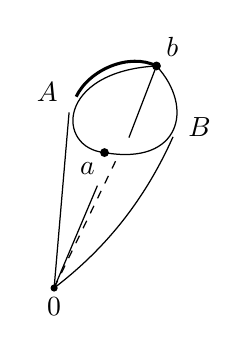
\begin{tikzpicture}[x=1cm,y=1cm,line width=.45pt]
\coordinate (o) at (0,0);
\coordinate (a) at (.64,1.72);
\coordinate (b) at (1.30,2.82);
\draw (a) .. controls (.02,1.78) and (.03,2.75) .. (b);
\draw[line width=1.1pt] (.28,2.43) .. controls (.45,2.78) and (.96,2.99) .. (b);
\draw (b) .. controls (1.79,2.29) and (1.60,1.55) .. (a);
\draw (o) -- (.19,2.23);
\draw (o) .. controls (.76,.58) and (1.21,1.25) .. (1.51,1.92);
\draw (b) -- (.95,1.91);
\draw[dashed] (o) -- (.78,1.61);
\draw (o) -- (.55,1.30);
\fill (a) circle (1.6pt);
\fill (b) circle (1.6pt);
\fill (o) circle (1.3pt);
\node[left] at (.17,2.49) {$A$};
\node[right] at (1.58,2.04) {$B$};
\node[below left] at (a) {$a$};
\node[above right] at (b) {$b$};
\node[below] at (o) {$0$};
\end{tikzpicture}}}

Pour tout $x\in X$, considérons \inserted{l'ens $I_x\subset I$} des $i\in I$ tels
que $X_i\ni x$ --- il y en a un nb fini, \deleted{et}
(par (1' a)), et l'ens de ces $\unsure{I|i}$ est filtrant
décroissant par (21 d), donc il y a
un plus petit $i\in I_x$ \deleted{tel que}, soit $i(x)$
\[
(25)\qquad i(x)=\text{plus petit des }i\in I\text{ tels que }x\in X_i.
\]
Soit d'autre part, pour tout $i\in I$
\mspage{53}
